\documentclass[11pt,a4paper]{scrartcl}
\usepackage[utf8]{inputenc}
\usepackage[T1]{fontenc}
\usepackage[ngerman]{babel}

\usepackage{paralist}
\usepackage{enumitem} 

%\usepackage {picins}

\usepackage{float}

% -- Mathe
%\usepackage{gensymb}
%fancyhdr, lastpage, booktabs, xy
\usepackage{graphicx}
\usepackage{amsmath}
\usepackage{amsfonts}
\usepackage{amssymb}
\usepackage{amsthm}
\usepackage{rotating}
\usepackage{hyperref}
\usepackage{mathtools}
\usepackage{marginnote}
\usepackage{MnSymbol}
 \usepackage[left=2cm,top=1.5cm,bottom=3cm,includeheadfoot]{geometry} 

% -- Malen
\usepackage{tikz}
\usetikzlibrary{patterns, decorations.pathreplacing, decorations.pathmorphing, arrows}
\usepackage{units}

\author{Philipp Beck}

\subtitle{Proseminar Funktionentheorie 2016 }
\title{Elliptische Funktionen}
%\\
% Die Sätze von Liouville und die Weierstraßsche Konstruktion elliptischer Funktionen}
\date{12. Mai 2016}

\renewcommand{\Re}{\operatorname{Re}}
\renewcommand{\Im}{\operatorname{Im}}
\newcommand{\Bild}{\operatorname{Bild}}

\newcommand{\Res}{\operatorname{Res}}
\newcommand{\ord}{\operatorname{ord}}

\newcommand{\td}[1]{\text{\rmfamily d} #1}

%\renewcommand\qedsymbol{$\blacksquare$}



\newtheoremstyle{mydef}
  {\topsep}% Platzhalter nach oben
  {\topsep}% Platzhalter nach unten
  {\normalfont}% Schriftart im Theoremkörper
  {0pt}% Seitlicher Einschub
  {\bfseries}% Schriftart in der Theoremüberschrift
  {:\\}% Punkt zwischen Überschrift und Körper
  {5pt plus 1pt minus 1pt}% Platz nach überschrift mit 2pt Ausweichvermögen
  {}% Spezifikationen

\newtheoremstyle{mythm}
  {\topsep}% Platzhalter nach oben
  {\topsep}% Platzhalter nach unten
  {\normalfont}% Schriftart im Theoremkörper
  {0pt}% Seitlicher Einschub
  {\bfseries \itshape}% Schriftart in der Theoremüberschrift
  {:\\}% Punkt zwischen Überschrift und Körper
  {5pt plus 1pt minus 1pt}% Platz nach überschrift mit 2pt Ausweichvermögen
  {}% Spezifikationen

\newtheoremstyle{myproof}
  {\topsep}% Platzhalter nach oben
  {\topsep}% Platzhalter nach unten
  {\normalfont}% Schriftart im Theoremkörper
  {0pt}% Seitlicher Einschub
  {\bfseries }% Schriftart in der Theoremüberschrift
  {:\\}% Punkt zwischen Überschrift und Körper
  {5pt plus 1pt minus 1pt}% Platz nach überschrift mit 2pt Ausweichvermögen
  {}% Spezifikationen



\newcommand{\thistheoremname}{}
\swapnumbers

\newtheorem{sz}{Satz}[section]
\newtheorem{gsz}[sz]{\thistheoremname}

\theoremstyle{definition}
\newtheorem{df}[sz]{Definition}
\newtheorem{gd}[sz]{\thistheoremname}


\theoremstyle{myproof}

\newtheorem*{bw}{\textbf{Beweis}}


%\newenvironment{bw}[1][\textbf{Beweis}]{\begin{proof}[#1]}{\end{proof}}

\newenvironment{genericdef}[1]{\renewcommand{\thistheoremname}{#1}\begin{gd}}{\end{gd}}

\newenvironment{bla}[1]{\renewcommand{\thistheoremname}{#1}\begin{gsz}}{\end{gsz}}

\parindent0pt
\parskip1ex


%----Dokument----

\begin{document}

\maketitle

%\clearpage

\section{Grundlegende Definition und Eigenschaften}

\begin{df}\label{1.1}
Eine meromorphe Funktion $f : \mathbb{C} \to \hat{\mathbb{C}}:=\mathbb{C} \cup \lbrace\infty \rbrace$ heißt \textit{elliptisch} oder 
\textit{doppelperiodisch},
falls es Zahlen $\omega_1, \omega_2 \in \mathbb{C}$
mit $ \Im \nicefrac{\omega_1}{\omega_2} \neq 0$ gibt
und 
\begin{align*}
f(z+\omega_1) = f(z) = f(z+\omega_2) 
\end{align*}
für alle $z \in \mathbb{C}$ erfüllt ist.
\end{df}
\begin{figure}[h]
  \centering
    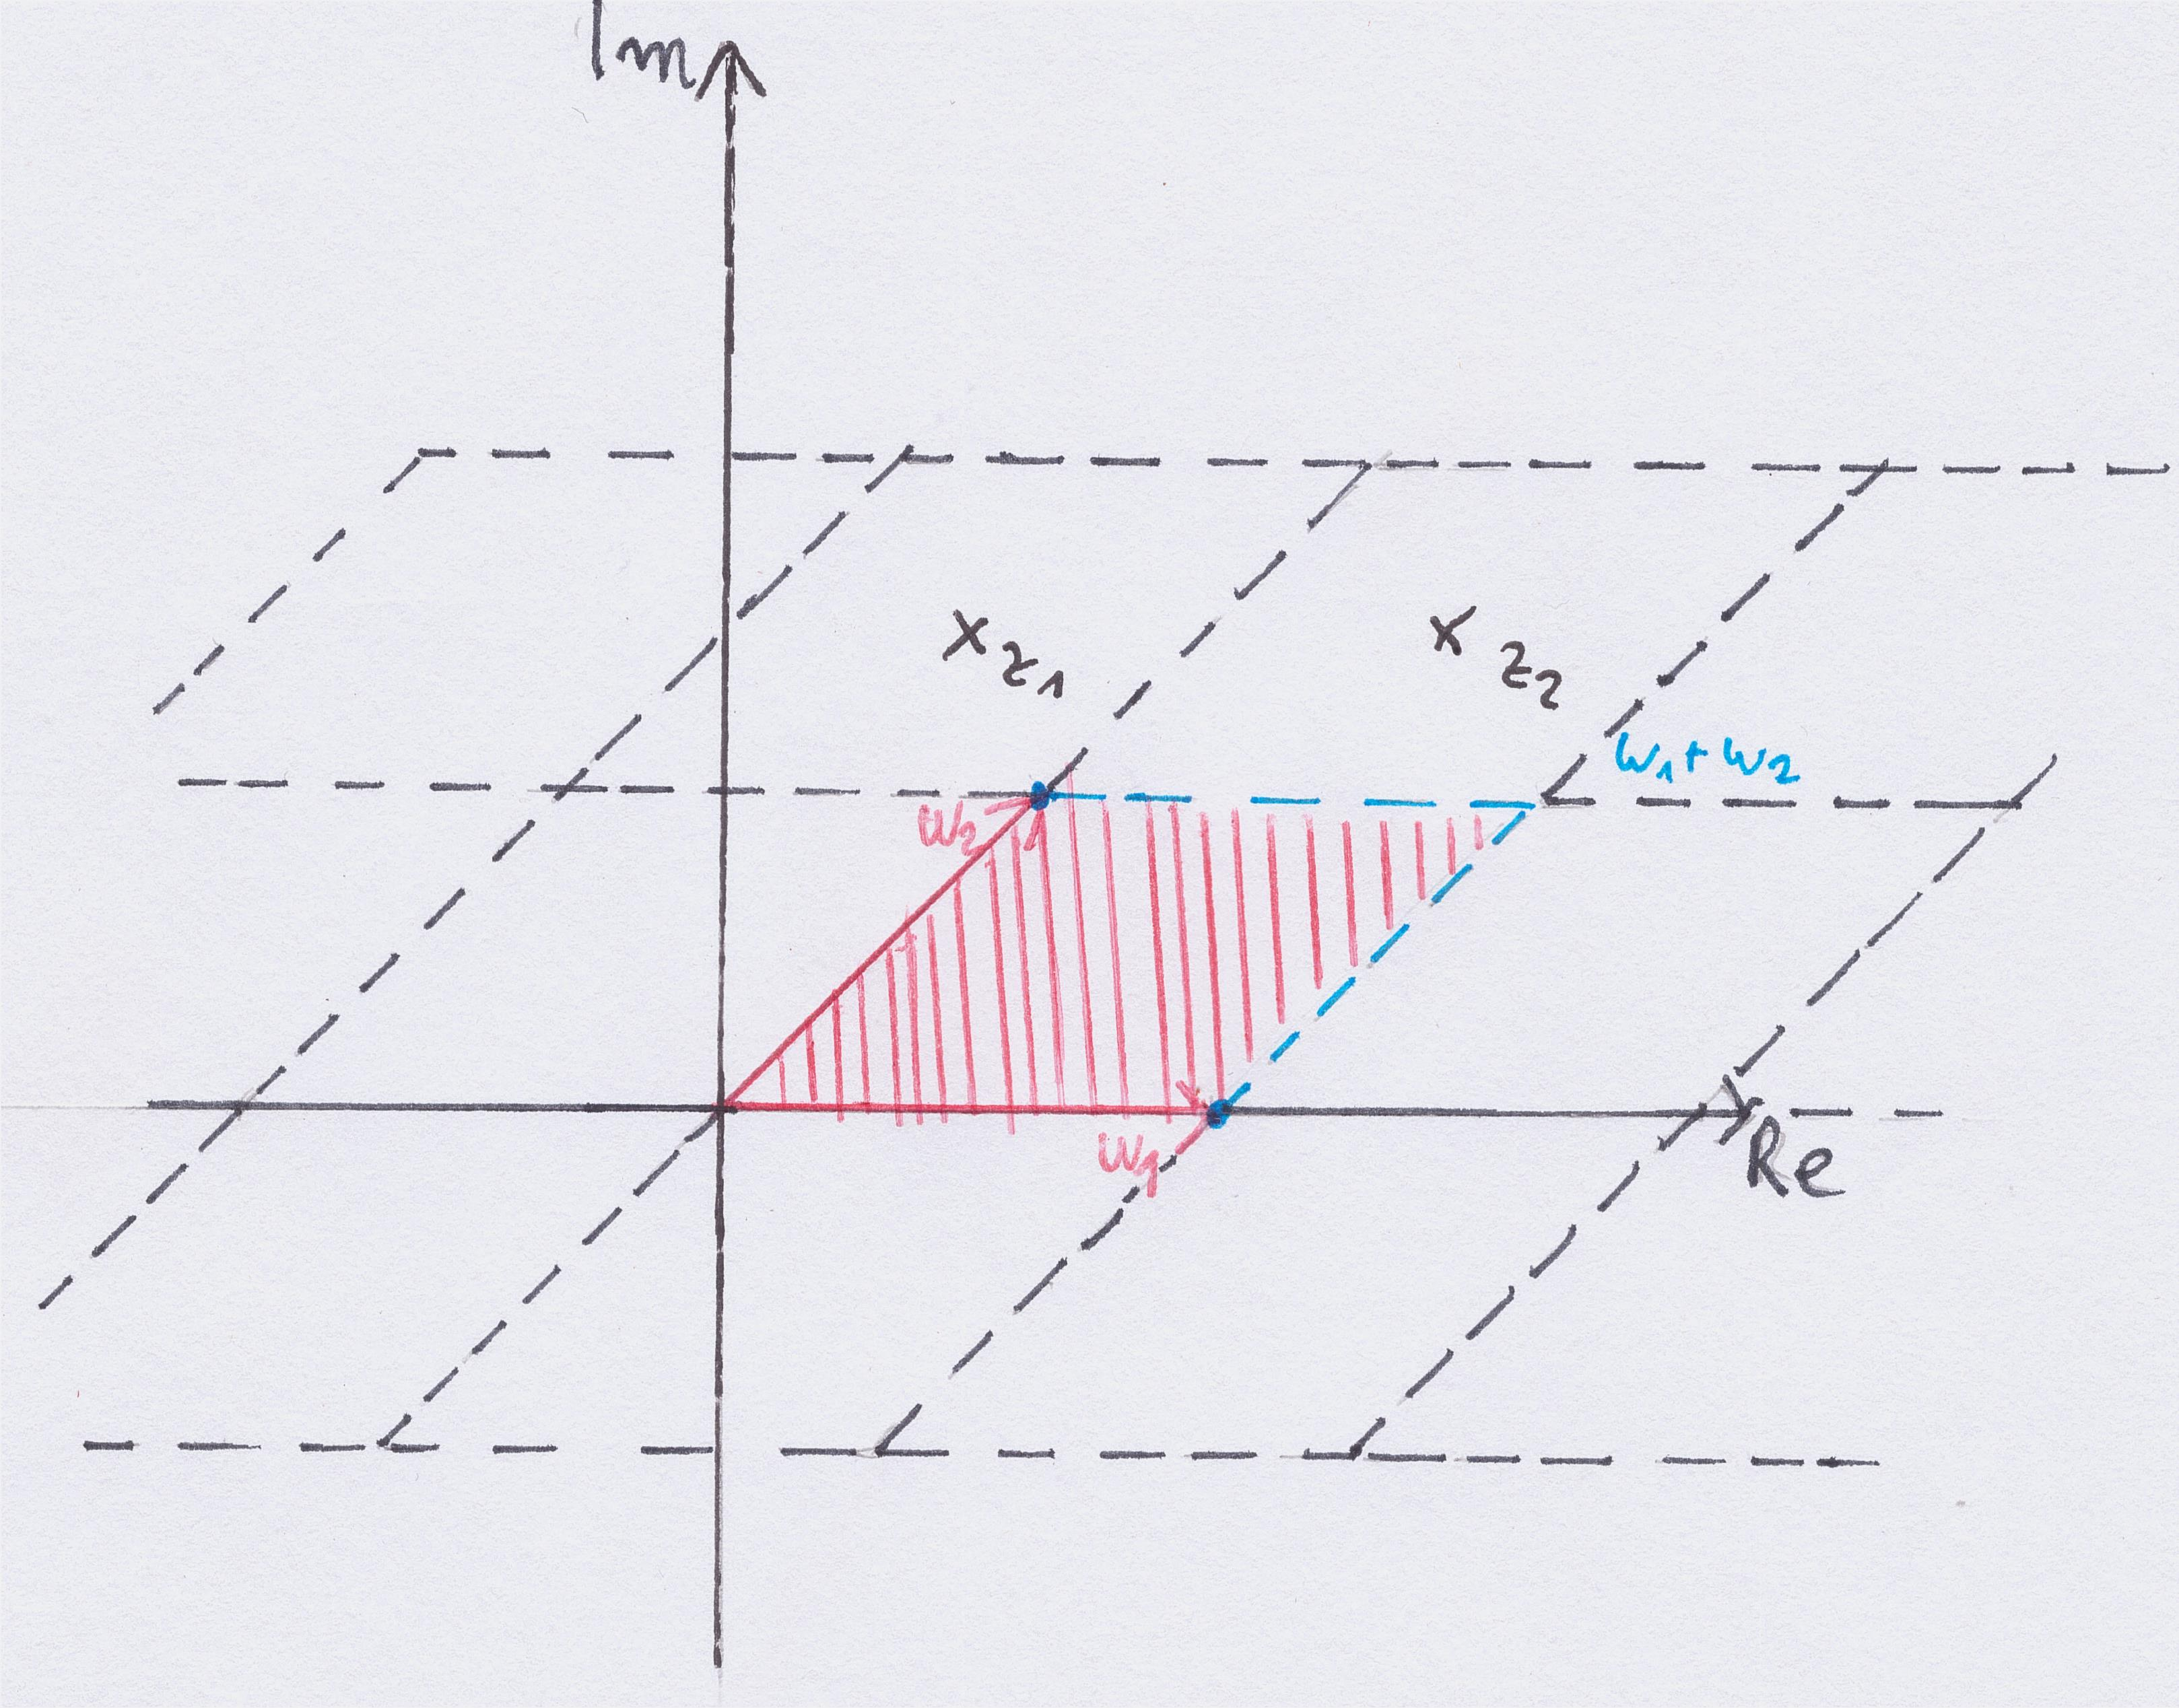
\includegraphics[width=0.65\textwidth]{sections/pics/Perioden}
  \caption{Beispiel eines Periodengitters}
\end{figure}
\begin{genericdef}{Periodenparallelogramm}\label{1.2}
Sei $f$ eine elliptische Funktion.
Das \textit{Periodengitter} von $f$ wird durch
\begin{align*}
\Gamma = \lbrace n \cdot \omega_1 + m \cdot \omega_2 \ | \ n,m \in \mathbb{Z} \rbrace
\end{align*}
beschrieben.
Da $\tau$ nicht reellwertig ist, spannen $\omega_1$ und $\omega_2$ ein Parallelogramm in der komplexen Ebene auf.
Zusätzlich setzt man $\Im \nicefrac{\omega_1}{\omega_2} < 0$ voraus,
damit die Eckpunkte $0$, $\omega_1$, $\omega_1+\omega_2$ und $\omega_2$ in einem positiven Sinn durchlaufen werden.
Nun besteht die Möglichkeit eine Äquivalenzrelation
\begin{align*}
z_1 \sim z_2 :\Leftrightarrow z_1-z_2 \in \Gamma
\end{align*}
zu definieren und die Funktion $f$ auf $\mathbb{C} / \Gamma$ zu betrachten.

Jede Äquivalenzklasse repräsentiert einen Punkt in dem aufgespannten Parallelogramm. Daraus erhält man, dass der blaue Teil des Randes nicht in dem Parallelogramm enthalten ist. Die Menge 
\begin{align*}
P := \lbrace  t \cdot \omega_1 + r \cdot \omega_2 \ | \ t,r \in [0,1) \rbrace
\end{align*} 
wird nun als \textit{Periodenparallelogramm} bezeichnet.
\begin{figure}[h]
  \centering
    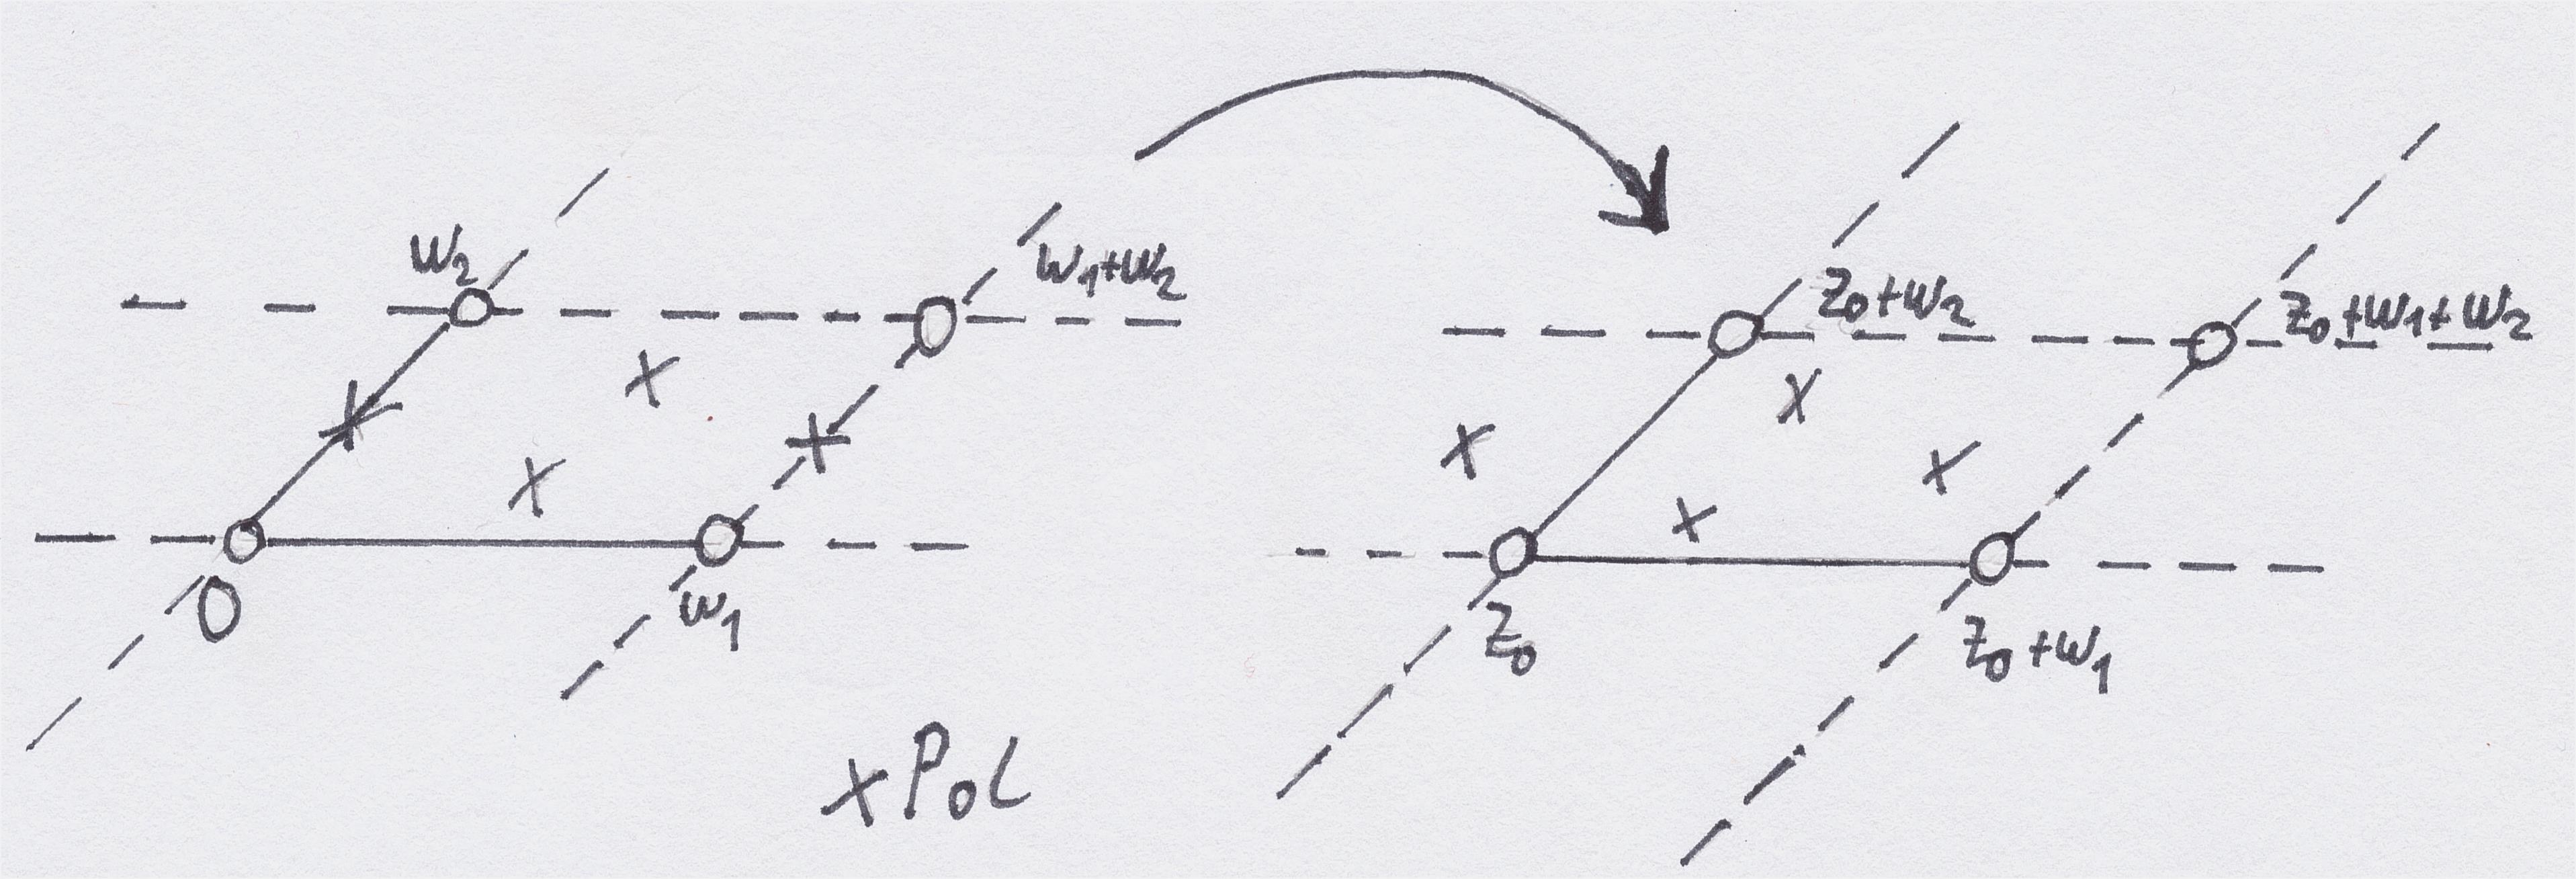
\includegraphics[width=0.80\textwidth]{sections/pics/verschiebung}
  \caption{Verschiebung}
\end{figure}
Für ein beliebiges $z_0 \in \mathbb{C}$
führt man mit
\begin{align*}
P_{z_o} := \lbrace z_0 + t \cdot \omega_1 + r \cdot \omega_2 \ | \ t,r \in [0,1) \rbrace
\end{align*}
eine \textit{Verschiebung des Periodenparallelogramms} ein.
Im weiteren Verlauf wird eine Eigenschaft oft innerhalb eines Periodenparallelogramms beschrieben. Dies bedeutet, dass eine Eigenschaft in einem beliebig verschobenen Periodenparallelogramm untersucht wird.
\end{genericdef}

\begin{df}\label{1.3}%Satz gefällt mir noch nicht.
Die \textit{Ordnung} $\ord(f)$ einer elliptischen Funktion $f$ ist die Anzahl der Pole unter Beachtung der Vielfachheit innerhalb eines Periodenparallelogramms.
\end{df}

\begin{sz}\label{1.4}
Seien $f,g,h$ elliptische Funktionen mit den Perioden $\omega_1, \omega_2$ und $ h\nequiv 0$ .
Dann sind $f + g$, $f \cdot g$, $\nicefrac{1}{h}$ und $f^\prime$ elliptische Funktionen mit den Perioden $\omega_1$ und $\omega_2$.
\end{sz}

\begin{proof}
%\begin{enumerate}[leftmargin=*]
%\item
Sei $z \in \mathbb{C}$ beliebig, wobei $z$ kein Pol von $f$ oder $g$ sein sollte.
Dann folgt sofort durch Nachrechnen:
\begin{align*}
(f+g)(z) = (f+g)(z+\omega_1)= (f+g)(z+\omega_2)
\end{align*}
Das Vorgehen ist für $f \cdot g$ und  $\nicefrac{1}{h}$ analog.
Bei $\nicefrac{1}{h}$ ist zu beachten, dass sich Null- und Polstellen vertauschen.
Man wird im weiteren Verlauf feststellen, dass dies die Ordnung nicht ändert.
%\item 
%Sei $z \in \mathbb{C}$ wieder beliebig und keine Polstelle von $f$.
Die Ableitung $f^\prime$ ist offenbar meromorph.
Weiter folgt mit der Identität aus Definition \ref{1.1} 
\begin{align*}
f^\prime(z+\omega_1) = f^\prime(z) = f^\prime(z+\omega_2) 
\end{align*}
und $f^\prime$ ist elliptisch.
%\end{enumerate}
\end{proof}


%\clearpage
\section{Die Liouvilleschen Sätze}

\begin{bla}{Erster Liouvillscher Satz}\label{2.1}
Sei $f : \mathbb{C} \to \mathbb{C}$ eine ganze Funktion.
Wenn $f$ elliptisch ist, dann ist $f$ konstant.
\end{bla}

\begin{proof}
Sei $f$ eine elliptische Funktion mit den Perioden $\omega_1$ und $\omega_2$.
Es genügt $f$ auf einem seiner Periodenparallelogramme zu betrachten.
Also betrachtet man die kompakte Menge
\begin{align*}
P := \lbrace t \cdot \omega_1 + r \cdot \omega_2 \ : \ t,r \in [0,1] \rbrace.
\end{align*}
und wählt $z \in P$ beliebig. Da $f$ holomorph auf $\mathbb{C}$ ist, ist $f$ stetig auf $P$.
Mit
\begin{align*}
| f(z) | \leq \max_{z \in P} |f(z)| < \infty.
\end{align*}
ist $f$ auf $P$ beschränkt. Aus der Periodizität folgt die Beschränkheit auf ganz $\mathbb{C}$.
Nach dem Satz von Liouville aus Analysis 3 ist $f$ damit konstant.
\end{proof}



\begin{bla}{Folgerungen}\label{2.2}
Aus dem vorherigen Satz ergeben sich die Folgerungen:
\begin{enumerate}%[leftmargin=*]
\item[\textbf{(1)} ]
Jede nicht konstante elliptische Funktion enthält in jedem Periodenparallelogramm mindestens 
einen Pol.
\item[\textbf{(2)}]
Seien $f $ und $g$ elliptische Funktionen mit den gleichen Perioden.
Zusätzlichen seien deren Polstellen und zugehörige Hauptteile identisch.
Dann ist $f-g $ konstant.
\item[\textbf{(3)}]
Seien $f $ und $g$ elliptische Funktionen mit den gleichen Perioden.
Nun seien die Null-und Polstellen und deren Ordnungen gleich.
Dann ist $\nicefrac{f}{g} $ konstant.
\end{enumerate}
\end{bla}

\begin{proof}
\begin{enumerate}%[leftmargin=*]
\item[(1)]
Mit der Annahme, dass $f$ keine Polstellen besitzt, erhält man mit \ref{2.1}
einen Widerspruch. 
\item[(2)]
Seien $f,g$ elliptische Funktionen mit den angegebenen Voraussetzungen. Dann ist auch $f-g$ elliptisch.
Nun sei $z_0$ eine beliebige Polstelle von $f$ und $g$ mit Ordnung $K$. Dann lassen sich $f,g$ in $z_0$ als Laurentreihe darstellen. Es gilt also:
\begin{align*}
f(z)-g(z)
= &\sum_{k=1}^K a_{-k} \cdot (z-z_0)^{-k} + \sum_{k=0}^\infty a_k \cdot (z-z_0)^k
- \sum_{k=1}^K b_{-k} \cdot (z-z_0)^{-k} - \sum_{k=0}^\infty b_k \cdot (z-z_0)^k\\
= &\sum_{k=0}^\infty (a_k -b_k) \cdot (z-z_0)^k
\end{align*} 
%Da die Haupteile gleich sind gilt: $\forall k \in \lbrace 1,...,K \rbrace : a_{-k} = b_{-k}$
Damit besitzt $f-g$ an $z_0$ eine hebbare Singularität und da $z_0$ beliebig gewählt wurde ist $f-g$ auf ganz $\mathbb{C}$ holomorph fortsetzbar. %\\
Also ist $f-g$ mit \ref{2.1} konstant.  
\item[(3)]
Seien $f,g$ elliptische Funktionen mit den angegebenen Voraussetzungen. Dann ist auch $\nicefrac{f}{g}$ elliptisch.
Nun kürzen sich Pole und Nullstellen gegenseitig weg. Damit besitzt $\nicefrac{f}{g}$
keine Pole.
Somit ist $\nicefrac{f}{g}$ mit \ref{2.1} konstant.
\end{enumerate}
\end{proof}

\begin{bla}{Zweiter Liouvillscher Satz}\label{2.3}
Sei $f$ eine elliptische Funktion mit den Perioden $\omega_1,\omega_2$.
Weiter sei $S$ die Menge der Polstellen innerhalb eines Periodenparallelogramms von $f$. Dann gilt
\begin{align*}
\sum \limits_{z \in S } \Res(f,z) = 0.
\end{align*} 
\end{bla}

\begin{proof}
Zunächst platziert man ein Periodenparallelogramm,
so dass keine Polstellen von $f$ auf dessen Rand liegen.
Nun betrachtet man
\begin{align*}
\gamma_1 &:= [z_0,z_0+\omega_1]\\
\gamma_2 &:= [z_0+\omega_1,z_0+\omega_1+\omega_2]\\
\gamma_3 &:= [z_0+\omega_1+\omega_2,z_0+\omega_2]\\
\gamma_4 &:= [z_0+\omega_2,z_0]
\end{align*}
und erhält den Weg 
$\gamma := \gamma_1 \cup \gamma_2 \cup \gamma_3 \cup \gamma_4$,
welcher das verschobene Parallelogramm berandet.
Zusätzlich fällt mit der Periodizität von $f$ auf, dass 
\begin{align*}
\int \limits_{\gamma_3} f(z) \ \td{z} = -\int \limits_{\gamma_1} f(z) \ \td{z}
\ \text{und} \
\int \limits_{\gamma_2} f(z) \ \td{z} = -\int \limits_{\gamma_4} f(z) \ \td{z}
\end{align*}
gilt.
Also folgt mit dem Residuensatz, dass
\begin{align*}
\int \limits_\gamma f(z) \ \td{z}
&= 2 \pi  \mathrm{i}  \cdot \sum \limits_{z \in S } \Res(f,z)\\
&= \int \limits_{\gamma_1} f(z) \ \td{z}
+ \int \limits_{\gamma_2} f(z) \ \td{z}
+ \int \limits_{\gamma_3} f(z) \ \td{z}
+ \int \limits_{\gamma_4} f(z) \ \td{z}\\
&= \int \limits_{\gamma_1} f(z) \ \td{z}
- \int \limits_{\gamma_1} f(z) \ \td{z}
- \int \limits_{\gamma_4} f(z) \ \td{z}
+ \int \limits_{\gamma_4} f(z) \ \td{z}
= 0
\end{align*}
ist. 
Somit gilt die Behauptung.
\end{proof}

\begin{bla}{Folgerung}\label{2.4}
Es existiert keine elliptische Funktion $f$ mit $\ord(f) = 1$.
\end{bla}
\begin{proof}
Angenommen eine solche Funktion $f$ würde existieren.
Dann gibt es innerhalb eines Periodenparallelogramms
genau einen Pol $z_0$ erster Ordnung. Also gilt $\Res(f,z_0) \neq 0$.
Dies steht im direktem Widerspruch zum letzten Satz.
\end{proof}

\begin{bla}{Dritter Liouvillscher Satz}\label{2.5}
Sei $f$ eine elliptische Funktion mit $\ord(f) = n \geq 2$. In einem beliebig verschobenen Periodenparallelogramm $P_{z_0}$ gilt für ein festes $a \in \mathbb{C}$
\begin{align*}
\# \lbrace z \in P_{z_0} \ | \ f(z) - a = 0   \rbrace  = n,
\end{align*}
wobei bezüglich der Vielfachheit gezählt wird.
Das heißt, in $P_{z_0}$ wird jeder Funktionswert $a \in \mathbb{C}$ genau $n$-mal 
angenommen.
\end{bla}

\begin{proof}
Sei $a \in \mathbb{C}$ beliebig aber fest.
Nun betrachtet man $f(z) - a$ und verschiebt ein Periodenparallelogramm so, 
dass keine Urbilder von $a$ auf dessen Rand liegen.
Dazu wählt man dann den Weg $\gamma$ aus \ref{2.4} .
Mit \ref{1.4} ist auch $\nicefrac{f^\prime(z)}{f(z)-a}$ eine elliptische Funktion.
Es folgt mit dem Null- und Polstellen zählenden Integral,
\begin{align*}
\frac{1}{2 \pi \mathrm{i}} \cdot \int \limits_\gamma \frac{f^\prime(z)}{f(z)-a} \ \td{z}
= N - P \overset{\ref{2.4}}{=} 0
\quad \Longrightarrow \quad N = P
\end{align*}
wobei $N$  die Anzahl der Nullstellen von $f(z) - a$, also die Anzahl der Urbilder von $a$ unter $f$ ist und $P = n$
gilt.
Damit wird $a$ genau $n$-mal innerhalb eines Periodenparallelogramms angenommen.
\end{proof}

\begin{genericdef}{Bemerkung}\label{2.6}
Seien die Voraussetzungen wie im letzten Satz.
Dann entspricht die Anzahl der Nullstellen von $f$ (mit Vielfachheiten gezählt) der Ordnung von $f$.
Also gilt $ \ord f = \ord \nicefrac{1}{f}$.
\end{genericdef}
%\clearpage
\section{Konstruktion der Weierstraßschen $\wp$-Funktion }


Seien $\omega_1, \omega_2 \in \mathbb{C}$ mit $ \Im \nicefrac{\omega_1}{\omega_2}  < 0$  fest vorgegeben. 
Sei weiter
\begin{align*}
\Gamma  := \omega_1 \mathbb{Z} + \omega_2 \mathbb{Z}
= \lbrace n \cdot \omega_1 + m \cdot \omega_2 \ | \ n,m \in \mathbb{Z}  \rbrace, 
\end{align*}
$\Gamma^\prime := \Gamma \setminus \lbrace 0 \rbrace$ und 
$S_R := \Gamma \cap \overline{B_R(0)} = \lbrace \omega \in \Gamma \ | \ |p| \leq R \rbrace$.


\begin{bla}{Hilfssatz}\label{3.1}
\begin{enumerate}%[leftmargin=*]
\item[\textbf{(1)}] 
Die Reihe
\begin{align*}
\sum \limits_{\omega \in \Gamma^\prime}  \frac{1}{\omega^3}
\end{align*}
konvergiert absolut. 
\item[\textbf{(2)})]
Die Reihe 
\begin{align*}
\sum \limits_{\omega \in \Gamma} \frac{1}{(z-\omega)^3}
\end{align*}
konvergiert für jedes $R>0$ auf $\overline{B_R(0)} \setminus S_R$ absolut und gleichmäßig.
\end{enumerate}
\end{bla}

\begin{proof}
\begin{enumerate}%[leftmargin=*]
\item[(1)]
Zunächst betrachtet man für $k \in \mathbb{N}$ den Weg $\gamma_k$
\begin{figure}[H]
  \centering
    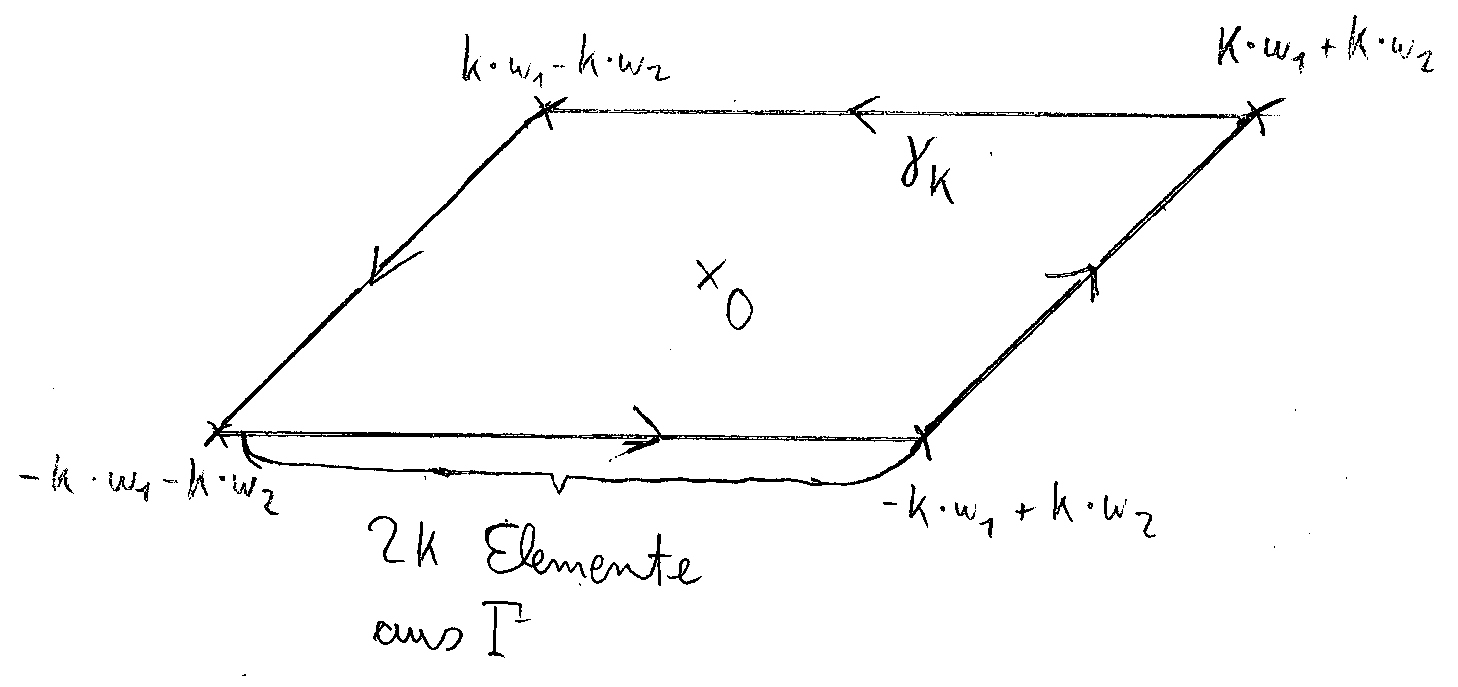
\includegraphics[width=0.60\textwidth]{sections/pics/weg}
  \caption{Der Weg $\gamma_k$}
\end{figure}
Für $\Pi_k := \gamma_k \cap \Gamma^\prime$ gilt dann 
\begin{align*}
\mathbin{\dot{\bigcup \limits_{k \in \mathbb{N}} }} \Pi_k = \Gamma^\prime
\ \text{und} \ | \Pi_k | = 8 \cdot k.
\end{align*}
Weiter bezeichnet man mit den $l$ den minimalen Abstand vom Ursprung zu den Elementen aus $\Pi_1$. Damit sind die Punkte in $\Pi_k$ minimal um $k \cdot l$ vom Ursprung entfernt.
\begin{figure}[H]
  \centering
    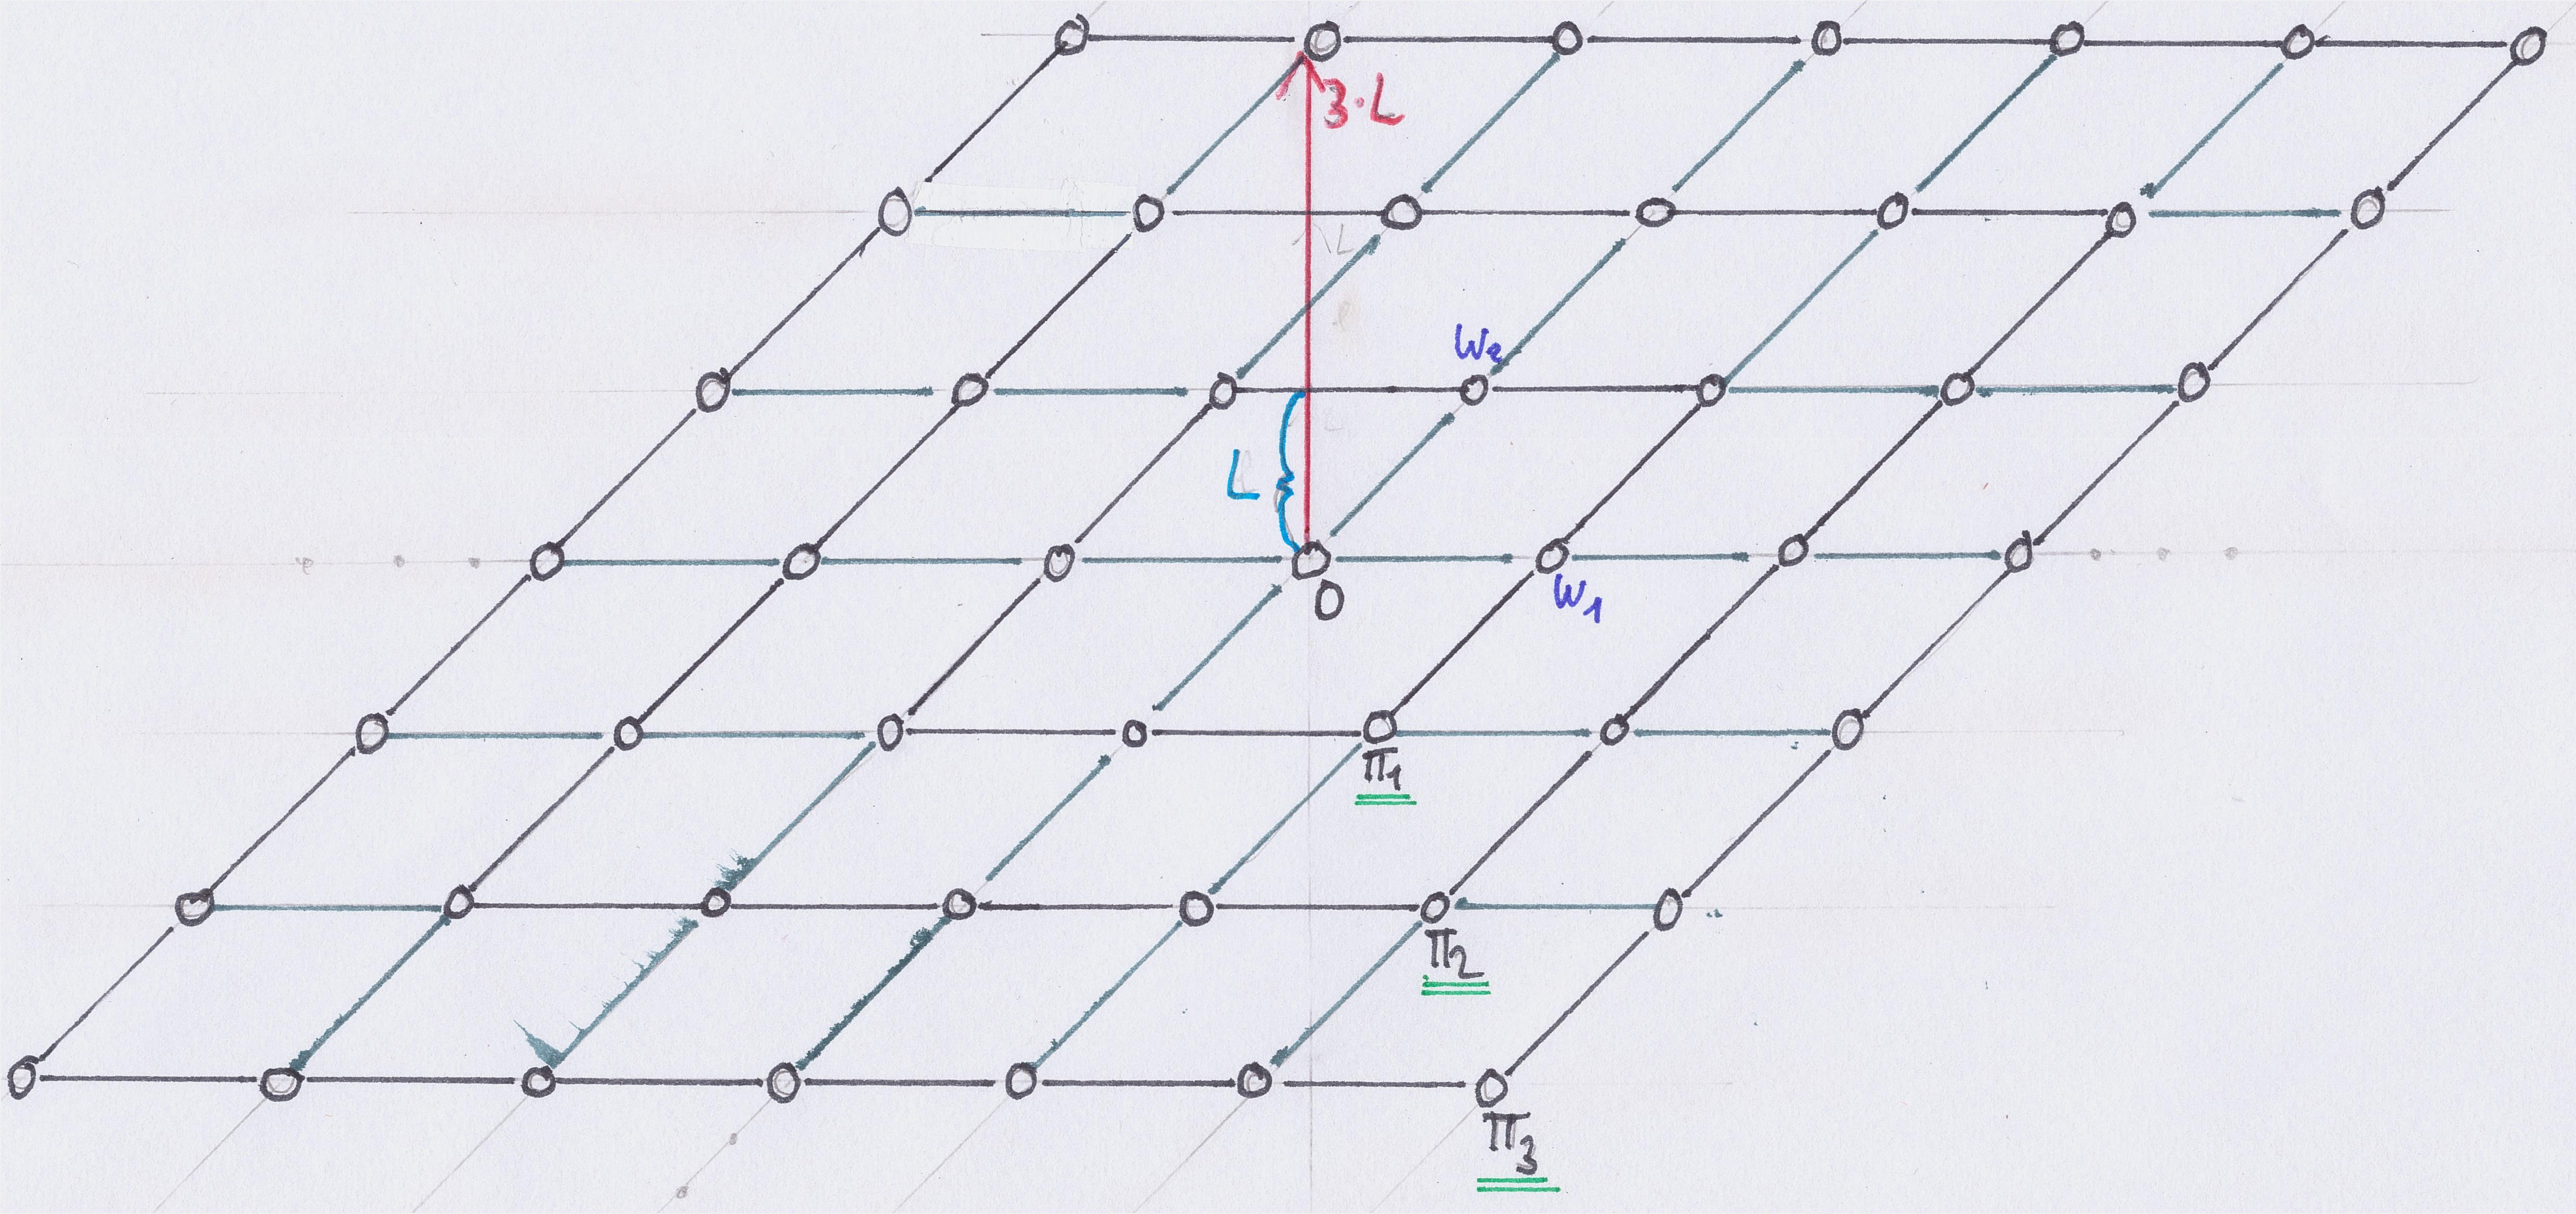
\includegraphics[width=0.80\textwidth]{sections/pics/gitter}
  \caption{Ausschnitt der Menge $\Gamma$}
\end{figure}
%Also enthält  die von $\gamma_k$ durchlaufene Punkte in $\Gamma^\prime$. Dies ist für $\Pi_1$, $\Pi_2$ und $\Pi_3$ in der Grafik zu sehen.
Mit diesen Überlegungen folgt dann
\begin{align*}
\sum \limits_{\omega \in \Gamma}  \frac{1}{|\omega|^3}
= \sum \limits_{k=1}^\infty \sum \limits_{\omega \in \Pi_k} \frac{1}{|\omega|^3}
\leq \sum \limits_{k=1}^\infty \frac{8 \cdot k}{|l \cdot k|^3}
= \frac{8}{l^3} \cdot \sum \limits_{k=1}^\infty \frac{1}{k^2}
< \infty
\end{align*}
und somit die absolute Konvergenz der Reihe.
\item[(2)]
In der Menge $ \overline{B_R(0)}$ liegen nur endlich viele Punkte aus $\Gamma$.
Diese sind gerade die Pole der Reihe, welche mit $S_R$ entfernt werden.
Sei also $z \in \overline{B_R(0)} \setminus S_R$ 
und $\omega \in \Gamma$ mit $|\omega| > 2 \cdot R$.
Damit erhält man die Abschätzung
\begin{align*}
\sum \limits_{|\omega| > 2R} \frac{1}{|(z-\omega)^3|}
&= \sum \limits_{|\omega| > 2R} \frac{1}{|\omega|^3 \cdot \left| (1- \frac{z}{\omega})\right|^3}
\leq \sum \limits_{|\omega| > 2R} \frac{1}{|\omega|^3 \cdot  \left(1- \frac{|z|}{|\omega|}\right)^3}
\leq \sum \limits_{|\omega| > 2R} \frac{1}{|\omega|^3 \cdot  \left(1- \frac{R}{2\cdot R}\right)^3}\\
&=  8 \cdot \sum \limits_{|\omega| > 2R} \frac{1}{|\omega|^3 }
\end{align*}
und mit \textbf{(1)} die absolute und gleichmäßige Konvergenz auf der Reihe.
\end{enumerate}
\end{proof}

\begin{genericdef}{Bemerkung}\label{3.2}
Die Reihe
\begin{align*}
\sum \limits_{\omega \in \Gamma^\prime}  \frac{1}{\omega^2}
\end{align*}
ist divergent.
(Dies folgt aus der Divergenz der harmonischen Reihe.)

\end{genericdef}

\begin{sz}\label{3.3}
Die Funktion
\begin{align*}
f(z) := \sum \limits_{\omega \in \Gamma} \frac{1}{(z-\omega)^3}
\end{align*}
ist elliptisch mit den Perioden $\omega_1$ und $\omega_2$ und der 
Ordnung $3$. Außerdem ist $f$ ungerade.
\end{sz}

\begin{proof}
Sei $R > 0$ beliebig aber fest.
Dann lässt sich $f$ für $z \in \overline{B_R(0)}$ in 
\begin{align*}
f(z) = \sum \limits_{|\omega| \leq R} \frac{1}{(z-\omega)^3} + \sum \limits_{|\omega|> R}  \frac{1}{(z-\omega)^3} 
\end{align*}
zerlegen. Für alle $\omega \in \Gamma$ mit $|\omega| \leq R$ besitzt $f$ einen Pol dritter Ordnung.
Der vordere Teil der Summe ist also meromorph.
Der hintere Teil ist für die gewählten $z$ holomorph. 
Die Konvergenz wurde schon in \ref{3.1} geklärt. 
Insgesamt folgt, dass $f$ eine meromorphe Funktion ist.

Sei $z \in \mathbb{C}$ beliebig. Für ein $\omega \in \Gamma$ ist auch $(\omega-\omega_1) \in \Gamma$.
Insbesondere findet dadurch nur eine Umordnung der Reihe statt, was wegen der absoluten Konvergenz kein Problem darstellt. 
Also gilt
\begin{align*}
f(z + \omega_1) 
= \sum \limits_{\omega \in \Gamma} \frac{1}{(z+\omega_1-\omega)^3}
= \sum \limits_{(\omega-\omega_1) \in \Gamma} \frac{1}{(z+\omega_1-\omega-\omega_1)^3}
= \sum \limits_{(\omega-\omega_1) \in \Gamma} \frac{1}{(z-\omega)^3}
=f(z).
\end{align*}
Analog verfährt man für $\omega_2$ und erhält $f(z + \omega_2)= f(z) $.
Nun folgt durch mehrfaches Anwenden dieser Identitäten, dass für $n,m\in \mathbb{Z}$
\begin{align*}
f( z + n \cdot \omega_1 + m \cdot\omega_2) = f(z)  
\end{align*}
gilt. Also besitzt $f$ die Perioden $\omega_1, \omega_2$ und das Periodengitter $\Gamma$.

Mit der absoluten Konvergenz gilt 
\begin{align*}
f(-z) 
= \sum \limits_{\omega \in \Gamma} \frac{1}{(-z-\omega)^3}
= -\sum \limits_{\omega \in \Gamma} \frac{1}{(z+\omega)^3}
= -\sum \limits_{-\omega \in \Gamma} \frac{1}{(z-(-\omega))^3}
=-f(z),
\end{align*}
womit $f$ ungerade ist.
\end{proof}


\begin{genericdef}{Konstruktion der Weierstraßschen $\wp$-Funktion}\label{3.4}
Seien $z_0,z  \in \mathbb{C} \setminus \Gamma$. Sei weiter $\gamma \subset \mathbb C\setminus \Gamma$ ein Weg, welcher $z_0$ und $z$ verbindet
und dabei keine Elemente aus $\Gamma$ trifft.
Nun gilt 
%\begin{align*}
$\Res(f,\omega) = 0$
%\end{align*}
für alle $\omega \in \Gamma$,
womit der konkrete Weg zwischen $z_0$ und $z$ keine Rolle spielt.
Dann erhält man durch gliedweise Integration die Funktion
\begin{align*}
\varphi(z) +C &= 
\int \limits_{\gamma} f(z)\  \td{z} 
= \sum \limits_{\omega \in \Gamma} \int \limits_{\gamma} \frac{1}{(z-\omega)^3} \ \td{z} 
= -\frac{1}{2} \cdot 
\sum \limits_{\omega \in \Gamma} \left(\frac{1}{(z-\omega)^2} -\frac{1}{(z_0-\omega)^2} \right) \\
&=-\frac{1}{2\cdot z^2} + \frac{1}{2 \cdot z_0^2} -\frac{1}{2} \cdot  \sum \limits_{\omega \in \Gamma^\prime} \left(\frac{1}{(z-\omega)^2} -\frac{1}{(z_0-\omega)^2} \right) 
\end{align*}
und durch Äquivalenzumformungen den Ausdruck
\begin{align*}
\varphi(z) + C + \frac{1}{2\cdot z^2}
= \frac{1}{2 \cdot z_0^2} -\frac{1}{2} \cdot  \sum \limits_{\omega \in \Gamma^\prime} \left(\frac{1}{(z-\omega)^2} -\frac{1}{(z_0-\omega)^2} \right).
\end{align*}
Die rechte Seite ist für $z = 0$ holomorph. Aus diesem Grund wählt man
\begin{align*}
C = \frac{1}{2 \cdot z_0^2} - \frac{1}{2} \cdot  
\sum \limits_{\omega \in \Gamma^\prime} \left(\frac{1}{\omega^2} -\frac{1}{(z_0-\omega)^2} \right)
\end{align*}
als Konstante und erhält durch Einsetzen
\begin{align*}
\varphi(z)
=-\frac{1}{2} \cdot \left(\frac{1}{z^2} + 
\sum \limits_{\omega \in \Gamma^\prime} \left( \frac{1}{(z-\omega)^2} - \frac{1}{\omega^2} \right) \right).
\end{align*}
Den Ausdruck innerhalb der äußeren Klammer bezeichnet man als \textit{Weierstraßsche $\wp$-Funktion} und kürzt diese mit
\begin{align*}
\wp(z) :=\frac{1}{z^2} + \sum \limits_{\omega \in \Gamma^\prime} \left( \frac{1}{(z-\omega)^2} - \frac{1}{\omega^2} \right)
\end{align*}
ab.
\end{genericdef}

%\begin{genericdef}{Bemerkung}\label{3.5}
%In der Herleitung von $\wp$ wurde die Wahl des Weges vom Punkt $z_0$ zu $z$ nur durch das Auslassen der Polstellen eingeschränkt.
%Mehr ist auch nicht notwendig, da 
%\begin{align*}
%\Res(f,\omega) = 0
%\end{align*}
%für alle $\omega \in \Gamma$ gilt.
%Somit spielt es keine Rolle wie oft ein Pol umlaufen wird oder an welcher 
%Seite eines Poles $\gamma$ entlangläuft. 
%\end{genericdef}

\begin{bla}{Eigenschaften der Weierstraßschen $\wp$-Funktion}\label{3.5}
Die Weierstraßsche $\wp$-Funktion 
\begin{align*}
\wp(z) =\frac{1}{z^2} + \sum \limits_{\omega \in \Gamma^\prime} \left( \frac{1}{(z-\omega)^2} - \frac{1}{\omega^2} \right)
\end{align*}
besitzt die folgenden Eigenschaften:
\begin{enumerate}%[leftmargin=*]
\item[\textbf{(1)}]
Die Reihe 
\begin{align*}
\sum \limits_{\omega \in \Gamma^\prime} \left( \frac{1}{(z-\omega)^2} - \frac{1}{\omega^2} \right)
\end{align*}
konvergiert für $z \in \mathbb{C} \setminus \Gamma$ absolut und lokal-gleichmäßig.
\item[\textbf{(2)}]
$\wp $ ist elliptisch mit den Perioden $\omega_1$ und $\omega_2$ und von der Ordnung 2.
\item[\textbf{(3)}]
$\wp$ ist gerade.
\end{enumerate}
\end{bla}

\begin{proof}
\begin{enumerate}%[leftmargin=*]
\item[(1)] 
Sei $R > 0$ beliebig. Dann existieren nur endlich viele $\omega \in \Gamma^\prime$ mit $|\omega| \leq 2R$.
Somit liefert, für $|\omega| > 2R$ und $z \in \overline B_R(0)$, die Abschätzung
\begin{align*}
\left| \frac{1}{(z-\omega)^2} - \frac{1}{\omega^2} \right|
&= \frac{|z| \cdot | 2 \cdot \omega -z|}{|z-\omega|^2 \cdot |\omega|^2}
\leq \frac{|z| \cdot  3 \cdot| \omega |}{|\omega-z|^2 \cdot |\omega|^2}
< \frac{R \cdot  3 \cdot| \omega |}{\left(|\omega|-|z|\right)^2 \cdot |\omega|^2}
< \frac{R \cdot  3 \cdot| \omega |}{\left(\frac{|\omega|}{2}\right)^2 \cdot |\omega|^2}\\
&= \frac{R \cdot  3 \cdot| \omega |}{\frac{|\omega|^2}{4} \cdot |\omega|^2}
=12 \cdot R \cdot \frac{1}{|\omega|^3}
\end{align*} 
nach \ref{3.1} eine konvergente Majorante. Somit folgt die absolute und lokal-gleichmäßige 
Konvergenz.

\item[(2)]
Mit der absoluten Konvergenz folgt für $z \in \mathbb{C} \setminus \Gamma$
\begin{align*}
\wp(-z) = \frac{1}{z^2} 
+ \sum \limits_{\omega \in \Gamma^\prime} \left( \frac{1}{(-z-\omega)^2}-\frac{1}{\omega^2} \right)
= \frac{1}{z^2} 
+ \sum \limits_{-\omega \in \Gamma^\prime} \left( \frac{1}{(z-(-\omega))^2}-\frac{1}{\omega^2} \right)
= \wp(z),
\end{align*}
womit $\wp$ gerade ist.

\item[(3)]
Aus der Konstruktion von $\wp$ ergibt sich $\wp^\prime(z) = -2\cdot f(z)$.
Also folgt mit \ref{2.3}, dass $\wp^\prime$ elliptisch mit den Perioden $\omega_1$ und $\omega_2$ ist.
Damit gilt dann
\begin{align*}
\wp^\prime(z+\omega_1)-\wp^\prime(z) = \wp^\prime(z+\omega_2)-\wp^\prime(z) = 0
\end{align*}
und mit Integration folgt
\begin{align*}
\wp(z+\omega_1)-\wp(z) = C_1 \ \text{und} \ \wp(z+\omega_2)-\wp(z) = C_2.
\end{align*}
Setzt man nun $z = -\nicefrac{\omega_1}{2}$ ein, dann gilt
\begin{align*}
\wp\left(\frac{\omega_1}{2}\right)-\wp\left(-\frac{\omega_1}{2}\right)
= \wp\left(\frac{\omega_1}{2}\right)-\wp\left(\frac{\omega_1}{2}\right) = 0 \ 
\Rightarrow \ C_1 = 0,
\end{align*}
da $\wp$ ungerade ist. Für $\omega_2$ verfährt man analog.
Damit ist $\wp$ eine elliptische Funktion mit den Perioden $\omega_1$ und $\omega_2$.
Da $\wp$ in einem Periodenparallelogramm eine Pol zweiter Ordnung enthält, hat $\wp$ die Ordnung $2$.
\end{enumerate}
\end{proof}

\begin{sz}\label{3.6}
Eine gerade elliptische Funktion besitzt eine gerade Ordnung.
\end{sz}

\begin{proof}
Sei $f$ eine gerade elliptische Funktion. Falls $f$ konstant ist folgt die Aussage sofort. Andernfalls platziert man ein Periodenparallelogramm um den Ursprung und betrachtet darin die Nullstellen.
Da $f$ gerade ist, gibt es für jede Nullstelle in $(1)$ auch eine
Nullstelle in $(3)$ mit identischer Vielfachheit.
Genauso argumentiert man für $(2)$ und $(4)$.
Damit ergibt sich eine gerade Anzahl an Nullstellen bezüglich den Vielfachheiten. 
Falls der Ursprung eine Nullstelle von $f$ sein sollte, ist deren Vielfachheit gerade. 
\begin{figure}[H]
  \centering
    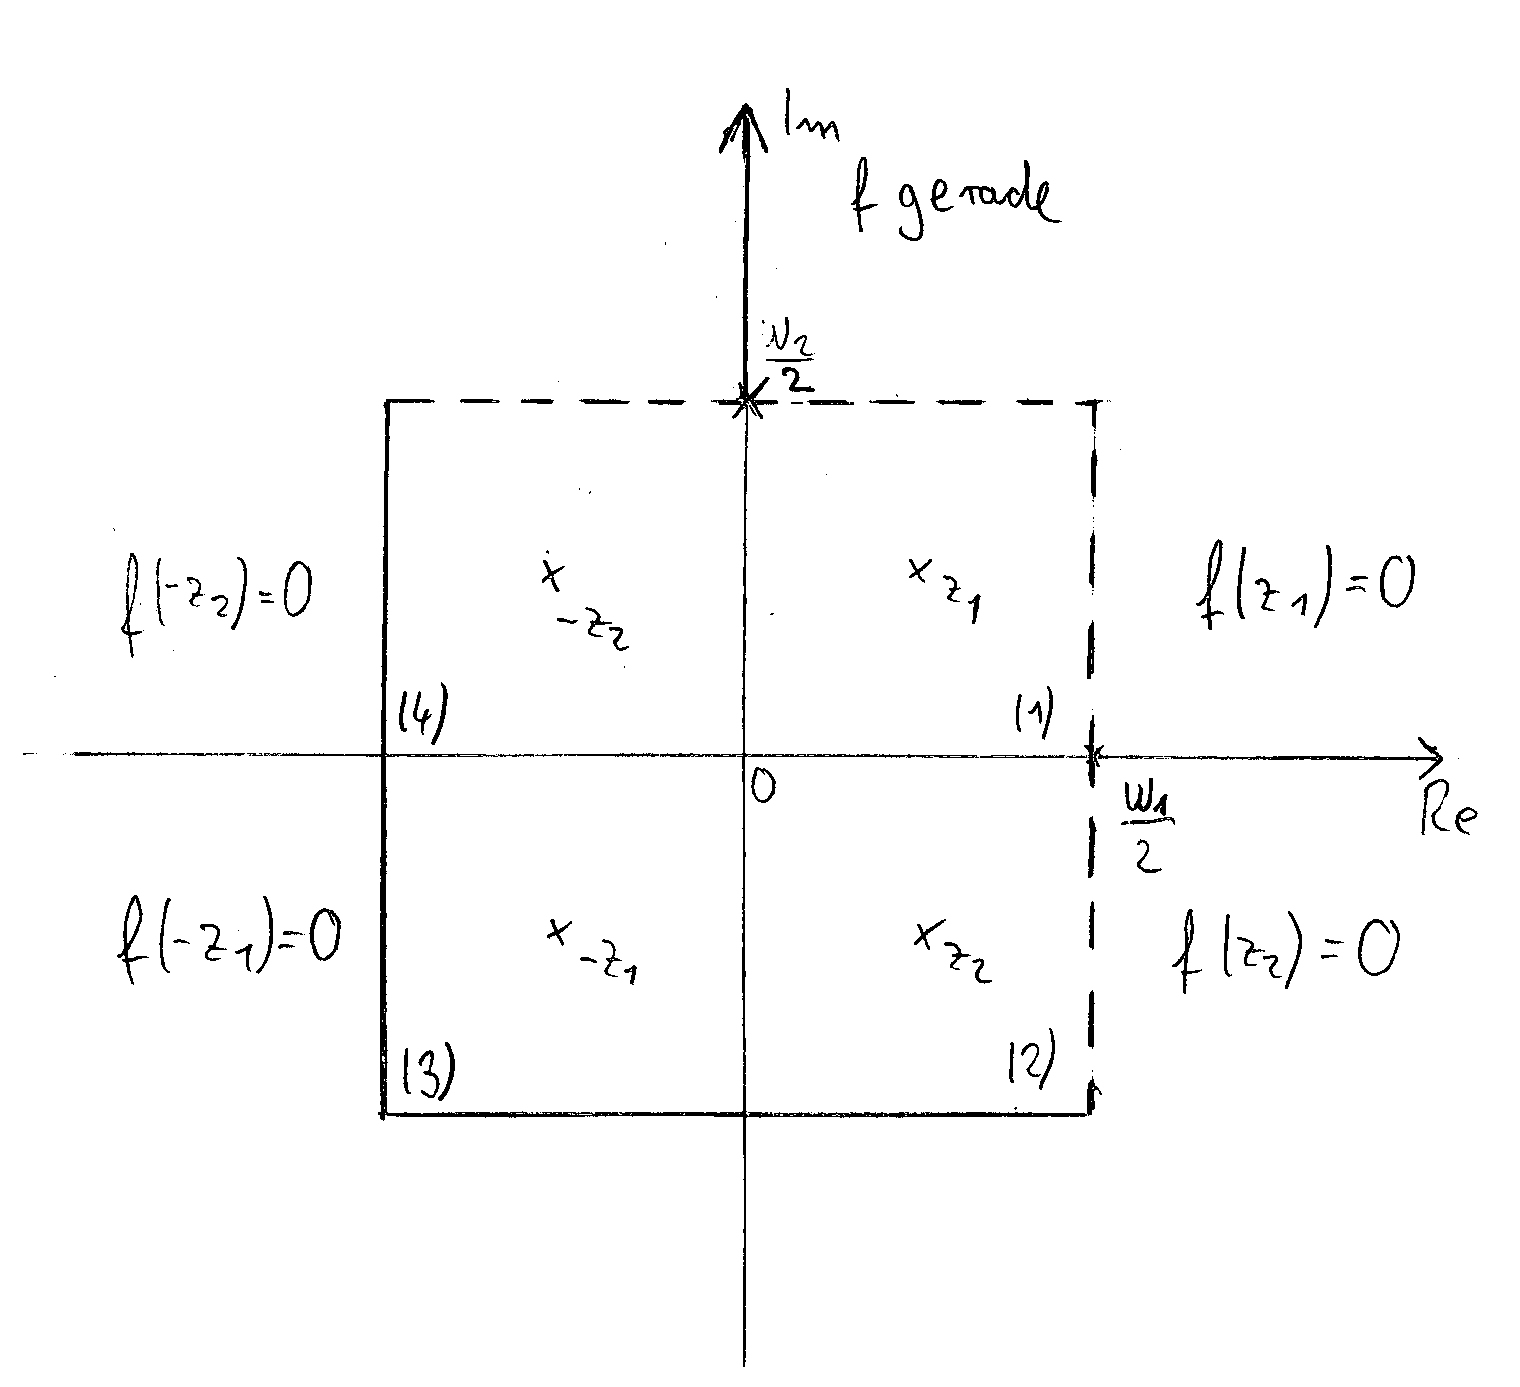
\includegraphics[width=0.62\textwidth]{sections/pics/ursprung}
  \caption{Periodenparallelogramm um den Ursprung}\label{ursprung}
\end{figure}
Insgesamt folgt also die Behauptung.
\end{proof}

\begin{sz}\label{3.7}
Sei $f$ eine gerade, elliptische Funktion mit den Perioden
$\omega_1,\omega_2$,
den Nullstellen $\pm a_1,..., \pm a_n$ 
und den Polstellen $\pm b_1,..., \pm b_n$. 
Dann lässt sich $f$ durch
\begin{align*}
f(z) = K \cdot \prod \limits_{r=1}^n \frac{\wp(z)-\wp(a_r)}{\wp(z)-\wp(b_r)}, \qquad K \in \mathbb{C},
\end{align*}
mit der Weierstraßschen $\wp$-Funktion darstellen,
wobei $\wp(z)-\wp(c) = 1$ für $c \in \Gamma$ gesetzt wird. 
\end{sz}

\begin{proof}
Nach \ref{3.6} ist die Ordnung von $f$ gerade mit den angegebenen Null- und Polstellen.
Die Funktion
\begin{align*}
\prod \limits_{r=1}^n \frac{\wp(z)-\wp(a_r)}{\wp(z)-\wp(b_r)}
\end{align*}
besitzt gerade diese Null- und Polstellen von $f$ mit identischen Vielfachheiten.
Nach \ref{2.2} ist 
\begin{align*}
\frac{1}{f(z)} \cdot \prod \limits_{r=1}^n \frac{\wp(z)-\wp(a_r)}{\wp(z)-\wp(b_r)}
\end{align*}
konstant. Somit folgt die Behauptung.
\end{proof}


\begin{bla}{Folgerung}\label{3.8}
Jede elliptische Funktion lässt sich mit der Weierstraßschen $\wp$-Funktion darstellen.
\end{bla}

\begin{proof}
Sei $f$ eine beliebige elliptische Funktion. Dann gilt
\begin{align*}
f(z) &= \frac{1}{2}\cdot (f(z) +f(-z)) + \frac{1}{2} \cdot (f(z)-f(-z))\\
&= \frac{1}{2}\cdot (f(z) +f(-z)) +\frac{1}{2} \cdot \frac{f(z)-f(-z)}{\wp^\prime(z)}\cdot \wp^\prime(z).
\end{align*}
$f(z) +f(-z)$ und $\nicefrac{f(z)-f(-z)}{\wp^\prime(z)}$ sind gerade. Wendet man \ref{3.7} hierauf an 
erhält man die Behauptung.
 \end{proof}

\begin{figure}[H]
  \centering
    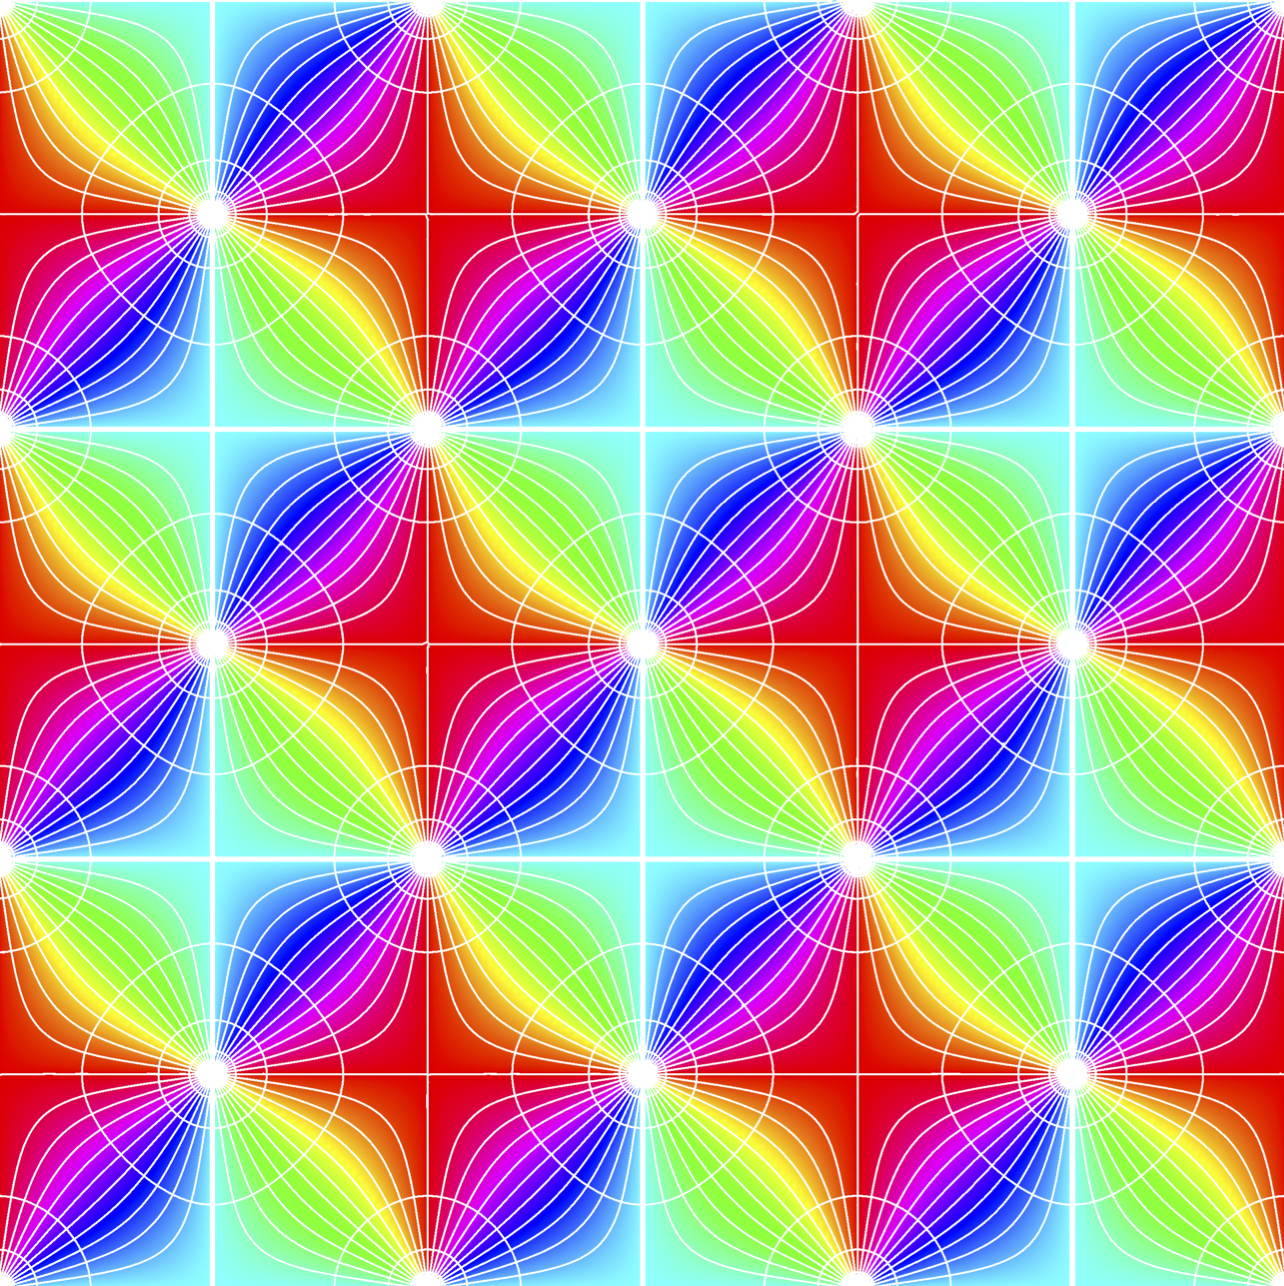
\includegraphics[width=0.49\textwidth]{sections/pics/weierstrassp}
  \caption{Die $\wp$-Funktion mit den Perioden $2$ und $2\mathrm{i}$ 
  mit Ursprung in der Mitte. }
\end{figure}

\end{document}
